\documentclass[../../thesis.tex]{subfiles}

\newcommand{\inner}[2]{\left<#1, #2\right>}
\newcommand{\alemap}{\ensuremath{\mathcal{A}}}
\newcommand{\dt}{\ensuremath{\Delta t}}
\newcommand{\pexp}{\ensuremath{\frac{2\gamma}{\left(\gamma-1\right)}}}
\newcommand{\aleX}{\ensuremath{\mathcal{X}}}
\newcommand{\Ah}[1]{\ensuremath{\vb{#1}^{n+1}_h}}
\newcommand{\Ahn}[1]{\ensuremath{\vb{#1}^{n}_h}}

\newcommand{\rbV}{\ensuremath{\mathbb{V}}}
\newcommand{\rbVT}{\ensuremath{\rbV^T}}
\newcommand{\epspod}{\ensuremath{\varepsilon_\text{POD}}}

\begin{document}

\section{Non-Hierachical POD Bases}
We investigate further the non-hierarchical character of the N-MDEIM basis.
After we linearized the nonlinear term, we obtained a trilinear form,
whose first two arguments are the usual test and trial functions,
with an additional third argument, used for the velocity extrapolation.

To build a basis, we proposed to obtain the snapshots from evaluations 
of the trilinear operator with RB elements,
\begin{equation}
    \begin{split}
        \qty[\Ah{N}\left(\psi_{h}\right)]_{i,j}
        &= b_0 \inner{\psi_h(x)\grad \varphi_j}{\varphi_i}^{n+1},
        \\[2mm]
        &= b_0 \int_{0}^{L(t^{n+1})} \psi_h(x) \grad \varphi_j \varphi_i \dd x.
    \end{split}
\end{equation}
Now, the reduced basis elements are expressed themselves in terms of 
the finite element Lagrangian basis functions,
\begin{equation}
    \psi_h(x) = \sum_{k} 
    \textcolor{blue}{\psi_k} 
    \varphi_{k}(x),
\end{equation}
which leads to the following exact expression for each of the entries of the nonlinear term,
\begin{equation}
    \begin{split}
        \qty[\Ah{N}\left(\psi_{h}\right)]_{i,j}
        &= b_0 \sum_k 
        \textcolor{blue}{\psi_k} 
        \underbrace{\int_{0}^{L(t^{n+1})} 
        \varphi_{k} \grad \varphi_j \varphi_i \dd x}_{\text{Only affected by $J(x, t)$}}.
    \end{split}
    \label{eq:appendix_exact_representation_triliear_form}
\end{equation}
Each summand is going to take a nonzero value only when the local support of the three
basis functions coincides simultaneously.

This approach lead to a non-hierarchical basis, 
of the same size as the number of RB elements it was fed with.
Why the basis is non-hierarchical could not be explained straightaway.

A detailed inspection of the matrix elements has not clarified our doubts.
During the assembly of the nonlinear operator during the FOM integration, 
the extrapolated velocity~$u^{*}$ is also expressed within the Lagrangian basis
(as shown in Equation~(\ref{eq:u_star_approximation}), 
it is a linear combination of the two previous timesteps).
And yet, the snapshots compressed from that source lead to a hierarchical reduced basis.
Therefore, the interaction between the finite element basis functions
does not seem to be the problem. 
There must be another effect playing a role 
in the non-hierarchical character of the reduced basis.

The remaining degrees of freedom are the coefficient values 
$\textcolor{blue}{\psi_k}$.
Since the solution is smooth,
when the snapshots are collected during the FOM simulation, 
each of the $u_k^{*}$ values is quite similar to the ones from the previous timestep.
However, when the reduced basis elements are used to create 
the nonlinear operator snapshots, 
for any two different basis elements $\psi_1(x)$ and $\psi_2(x)$,
we know that they satisfy an orthogonality condition,
\begin{equation}
    \int_\Omega \psi_1(x) \psi_2(x) \dd x = 0.
\end{equation}
We are going to explore if this condition is playing a role, 
by using as input functions elements from a naturally orthogonal basis:
the Fourier basis.
We do so to remove the complexity of the reduced basis construction 
(application of the POD on the solutions from the PDE). 

Our working hypothesis is that if the input functions used to evaluate the 
trilinear form are orthogonal, so will be the resulting POD base,
and hence non-hierarchical 
(there is no reduction capacity, since the input is already forming a base).

\subsection{Fourier Basis: Insights}
We kick-off by studying the effects of attempting an SVD over a Fourier basis, 
\begin{equation}
    \psi_q = \qty{\cos(2 \pi \omega_q x) \, : \, \omega_q \in \qty{1, \ldots, 3}}.
\end{equation}
We are going to carry out two experiments:
\begin{itemize}
    \item (I) Run the Fourier basis through the SVD and analyze its spectrum decay. 
    We would expect to find no decay at all, since the basis is orthogonal.
    \item (II) Compute snapshots of the nonlinear operator term with the Fourier basis
    and run them through the SVD as well.
    We shall look at the spectrum decay to establish conclusions. 
\end{itemize}

\subsubsection{(I) SVD of a Fourier Basis}
When the POD is applied to a naturally orthogonal basis, 
the resulting basis is formed by linear combinations of the input basis elements.

We recall that the POD is based on the SVD breakdown, which splits a matrix into 
two rotations and one scaling,
\begin{equation}
    A = U \Sigma V^T.
\end{equation}
If the matrix A is orthogonal ($AA^T = A^T A = I$),
we would expect that the transformation is such that the basis elements
remain unaltered,
$U=A, \Sigma = I,$ and $V=I$ 
(with their respective dimensions well set).
However, the only guarantee we can have is that $\Sigma = I$,
the rotations $U$ and $V$ are not unique.
And so is the case with the implementation we are using of the SVD.

Instead of returning the original Fourier basis, 
it is creating linear combinations of it, 
where the coefficients of the linear combination are collected in the columns of
\begin{equation}
    V = \begin{bmatrix}
        0.577 &  0     &  0.816 \\
        0.577 &  0.707 & -0.408 \\
        0.577 & -0.707 & -0.408 \\
    \end{bmatrix}.
\end{equation}
There is no spectrum decay, for all singular values are equal to $1.0$,
as shown in Table~\ref{tab:appendix_fourier_spectrum}.
\begin{table}[h]
    \centering
    \caption{Singular value spectrum for the SVD of the Fourier basis.
    Since the input is orthogonal, the resulting POD basis is non-hierarchical.
    To be aligned with the code, a 0-indexing presentation is used.}
    \begin{tabular}{cc}
        \toprule
        Singular index & $\sigma_i$ \\
        \midrule
        0 &  1.002 \\
        1 &  0.999 \\
        2 &  0.999 \\
        \bottomrule
    \end{tabular}
    \label{tab:appendix_fourier_spectrum}
\end{table}

\begin{figure}[h]
    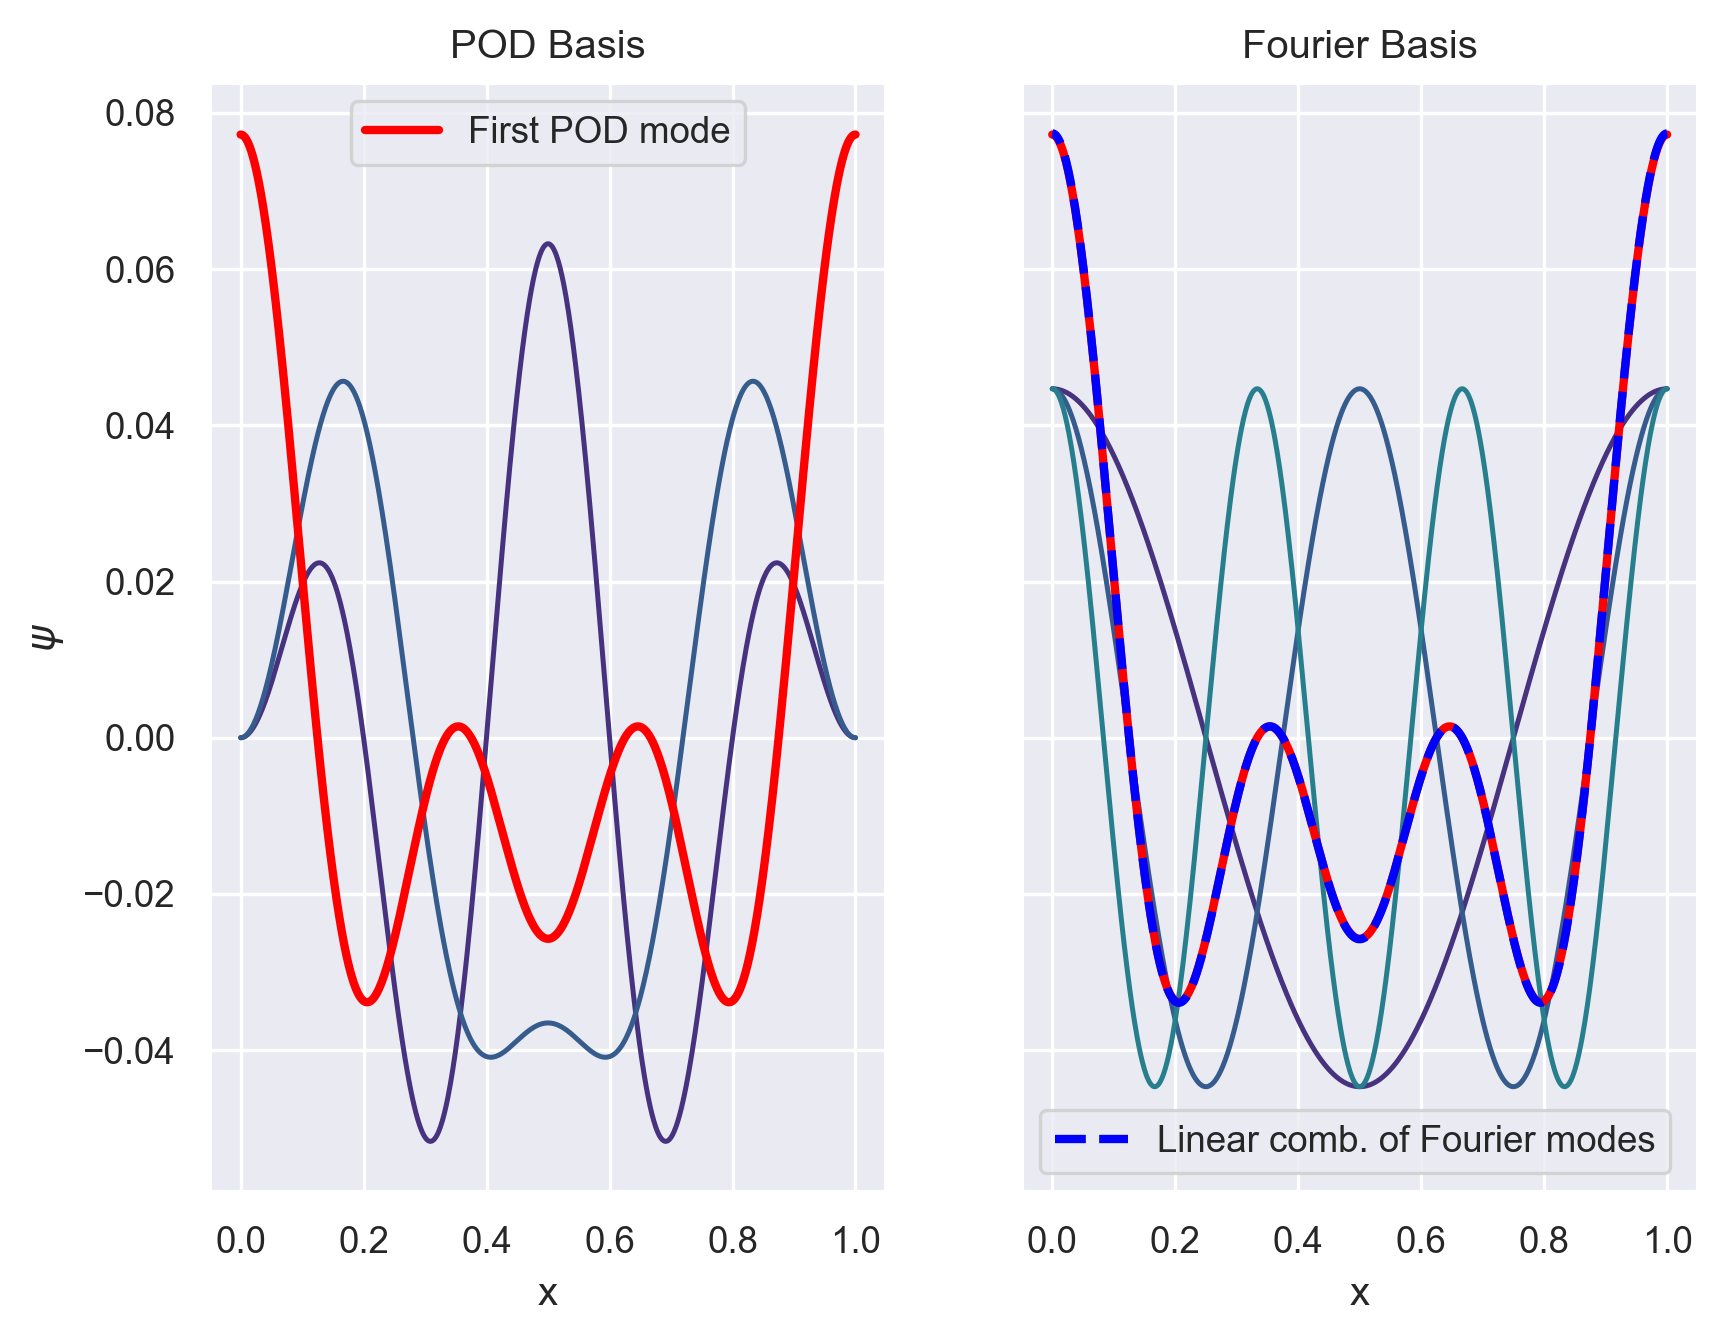
\includegraphics[width=\columnwidth]{research_project/piston/figures/svd_fourier/fourier_pod_bases.png}
    \caption{Fourier basis and its SVD transformation. 
    Since the Fourier basis is naturally orthogonal, 
    the resulting SVD transformation is simply a linear combination of Fourier modes.}
\end{figure}

\subsubsection{(II) N-MDEIM with Fourier Basis}
To confirm our working hypothesis, 
we build the trilinear form 
(Equation~(\ref{eq:appendix_exact_representation_triliear_form}))
using the first five elements of the Fourier basis,
\begin{equation}
    \psi_q(x) = \qty{\cos(2 \pi \omega_q x) \, : \, \omega_q \in \qty{1, \ldots, 5}}.
\end{equation}
Since the Jacobian transformation is a linear function of time, 
despite the change in time of the domain, the trilinear form remains linear.
If there were no third argument 
$\textcolor{blue}{\psi_k}$, 
we would only require one basis element to represent the whole operator.
Therefore, we predict that we will only find 5 orthogonal resulting modes, that is, a non-hierarchical basis. 
This is confirmed by the singular value decay, 
shown in Table~\ref{tab:ndeim_with_fourier_modes}
(to be aligned with the code, a 0-indexing presentation is used).

\begin{table}[h]
    \centering
    \caption{Singular value spectrum for the N-MDEIM reduction with a Fourier basis.
    We have built the snapshots in time for two parameters and five Fourier basis elements.
    Since we know the resulting bases will be of the same size as the original input,
    we expect to have only 5 non-zero singular values, which is the case.
    To be aligned with the code, a 0-indexing presentation is used.}
    \begin{tabular}{cc}
        \toprule
        Singular index & $\sigma_i$ \\
        \midrule
        0 &  1.414 \\
        1 &  1.414 \\
        2 &  1.414 \\
        3 &  1.414 \\
        4 &  1.414 \\
        5 &  0.000 \\
        6 &  0.000 \\
        7 &  0.000 \\
        8 &  0.000 \\
        9 &  0.000 \\
        \bottomrule
    \end{tabular}
    \label{tab:ndeim_with_fourier_modes}
\end{table}
Again, as depicted by Figure~\ref{fig:appendix_fourier_nmdeim_reconstruction_error},
we obtain the same poor results in the approximation error when
we attempt to reconstruct the operator with a truncated basis. 

\begin{figure}[h]
    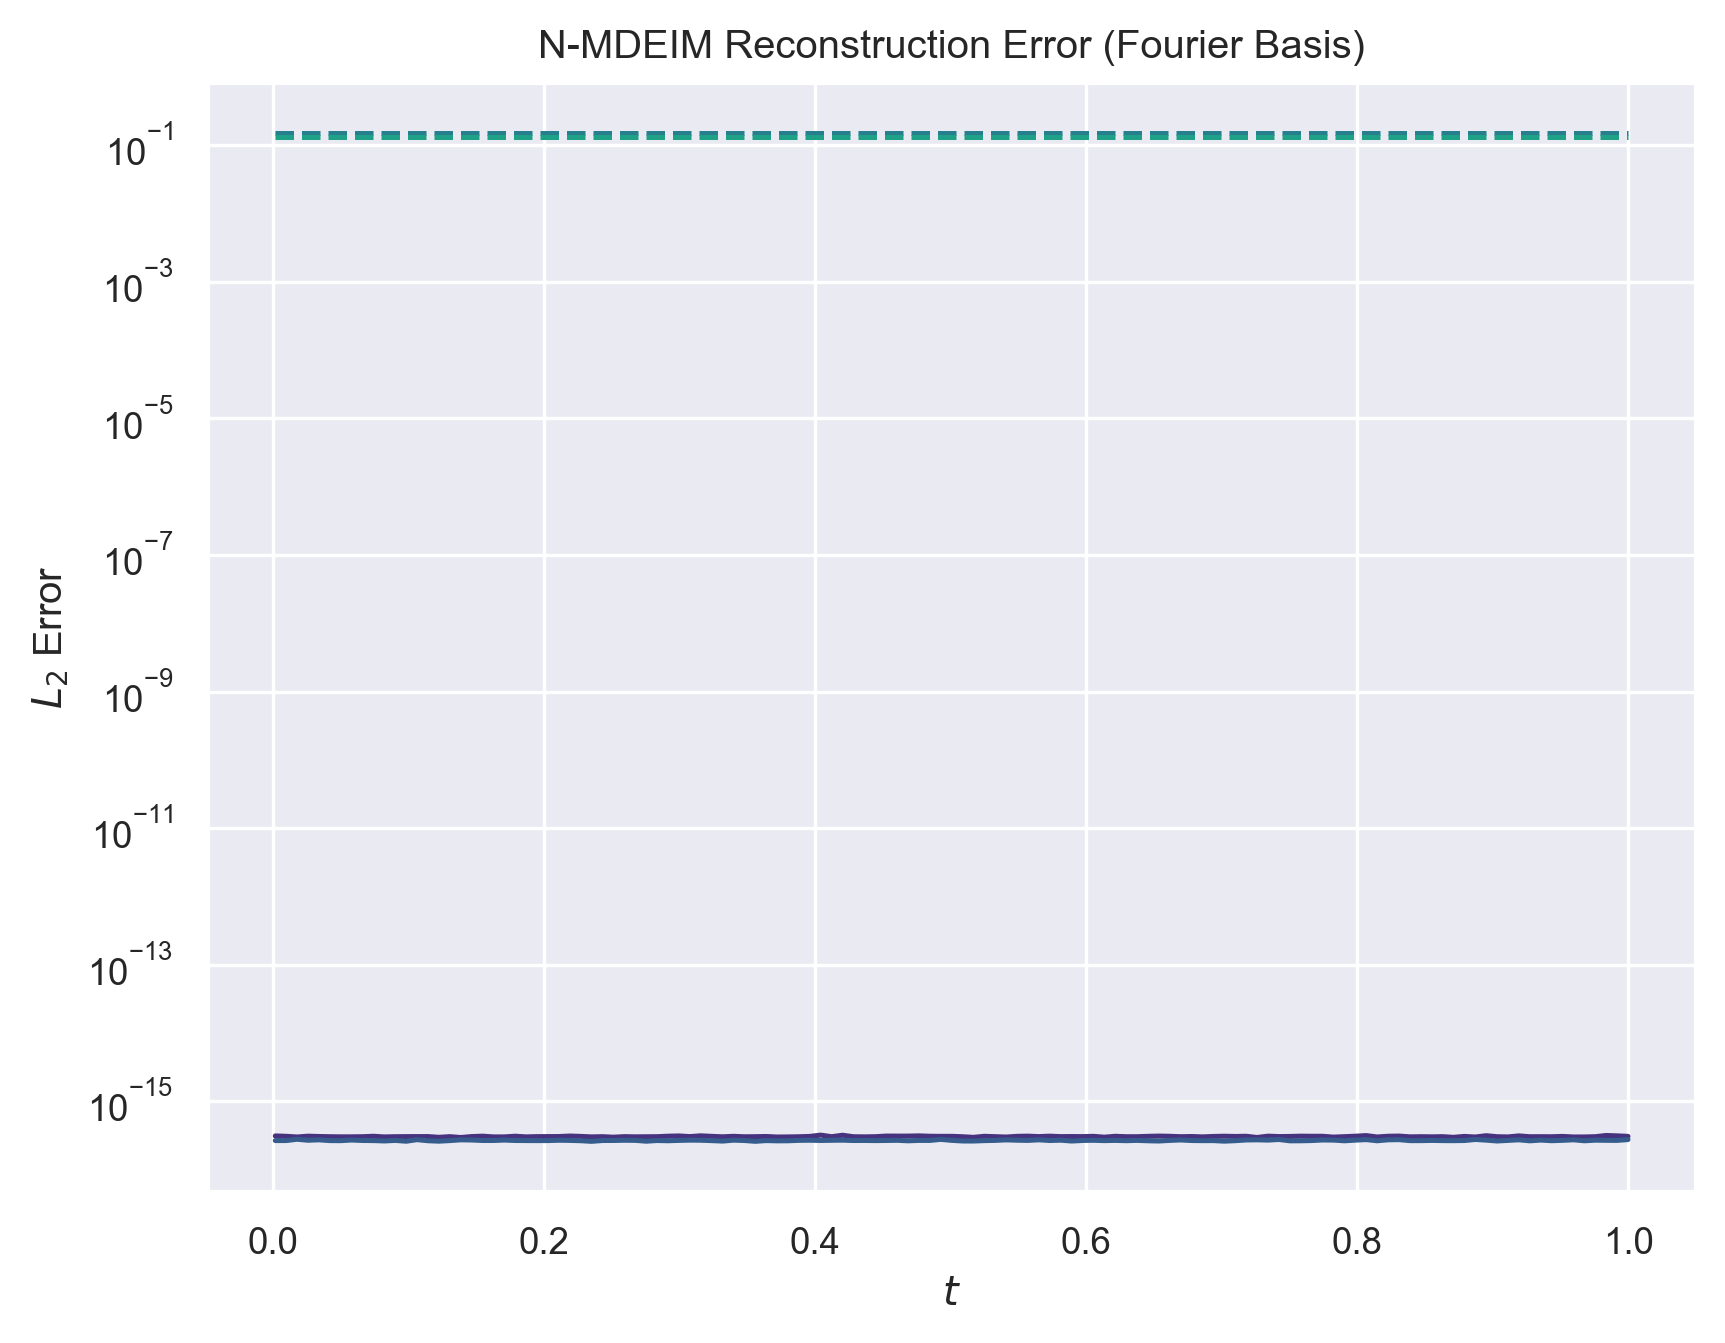
\includegraphics[width=\columnwidth]{research_project/piston/figures/svd_fourier/fourier_basis_mdeim_truncation_errors_comparison.png}
    \caption{N-MDEIM reconstruction error.
    The basis for this N-MDEIM has been built using 
    the first five Fourier basis elements to evaluate the trilinear form.
    According to the singular value decay, the basis is not hierarchical, 
    that is, all the basis elements (continuous) needs to be used to 
    create an accurate representation of the space.
    Hence, when one element is removed (dashed), 
    the approximation error increases to unaffordable values.}
    \label{fig:appendix_fourier_nmdeim_reconstruction_error}
\end{figure}

\subsection{N-MDEIM with One RB Element}
What would happen if we only used one basis element to reduce the operator?
Could we use that basis to approximate the trilinear operator evaluated with other functions?

We load the first three RB basis elements and create a function $f(x)$ as a linear combination of them,
\begin{equation}
    f(x) = 2 \psi_0(x) + \psi_1(x) + 3 \psi_0(x).
\end{equation} 
This is shown in Figure~\ref{fig:appendix_rb_linear_combination}.

We now reduce the trilinear form with two approaches:
\begin{itemize}
    \item (a) Subspace: using only the first RB mode.
    \item (b) Complete space: using all RB modes.
\end{itemize}

With each approach, we obtain a non-hierarchical orthogonal basis,
which we then use to reconstruct $\vb{N}_h\left(f(x)\right)$.
Since $f(x)$ is made out of the three orthogonal basis functions, 
we could expect approach (a) to fail.
However, it will succeed as well as approach (b).
This is proved by Figures~\ref{fig:appendix_rb_trilinear_num_1} 
and~\ref{fig:appendix_rb_trilinear_num_3}.
Additionally in Figure~\ref{fig:appendix_rb_trilinear_num_3} we have included 
the reconstruction error for the truncated base (we have removed one element). 

Using \textit{one} RB element is sufficient to construct a perfect collateral basis
due to the linearity of the integrand within the trilinear form 
and the linearity of the Jacobian transformation.
Despite the fact that the function $f(x)$ contains other modes, 
the collateral basis built with one mode is able to reproduce its effect on the operator perfectly. 

In the next section we explore what happens if a nonlinear Jacobian was present instead.
\begin{figure}[h]
    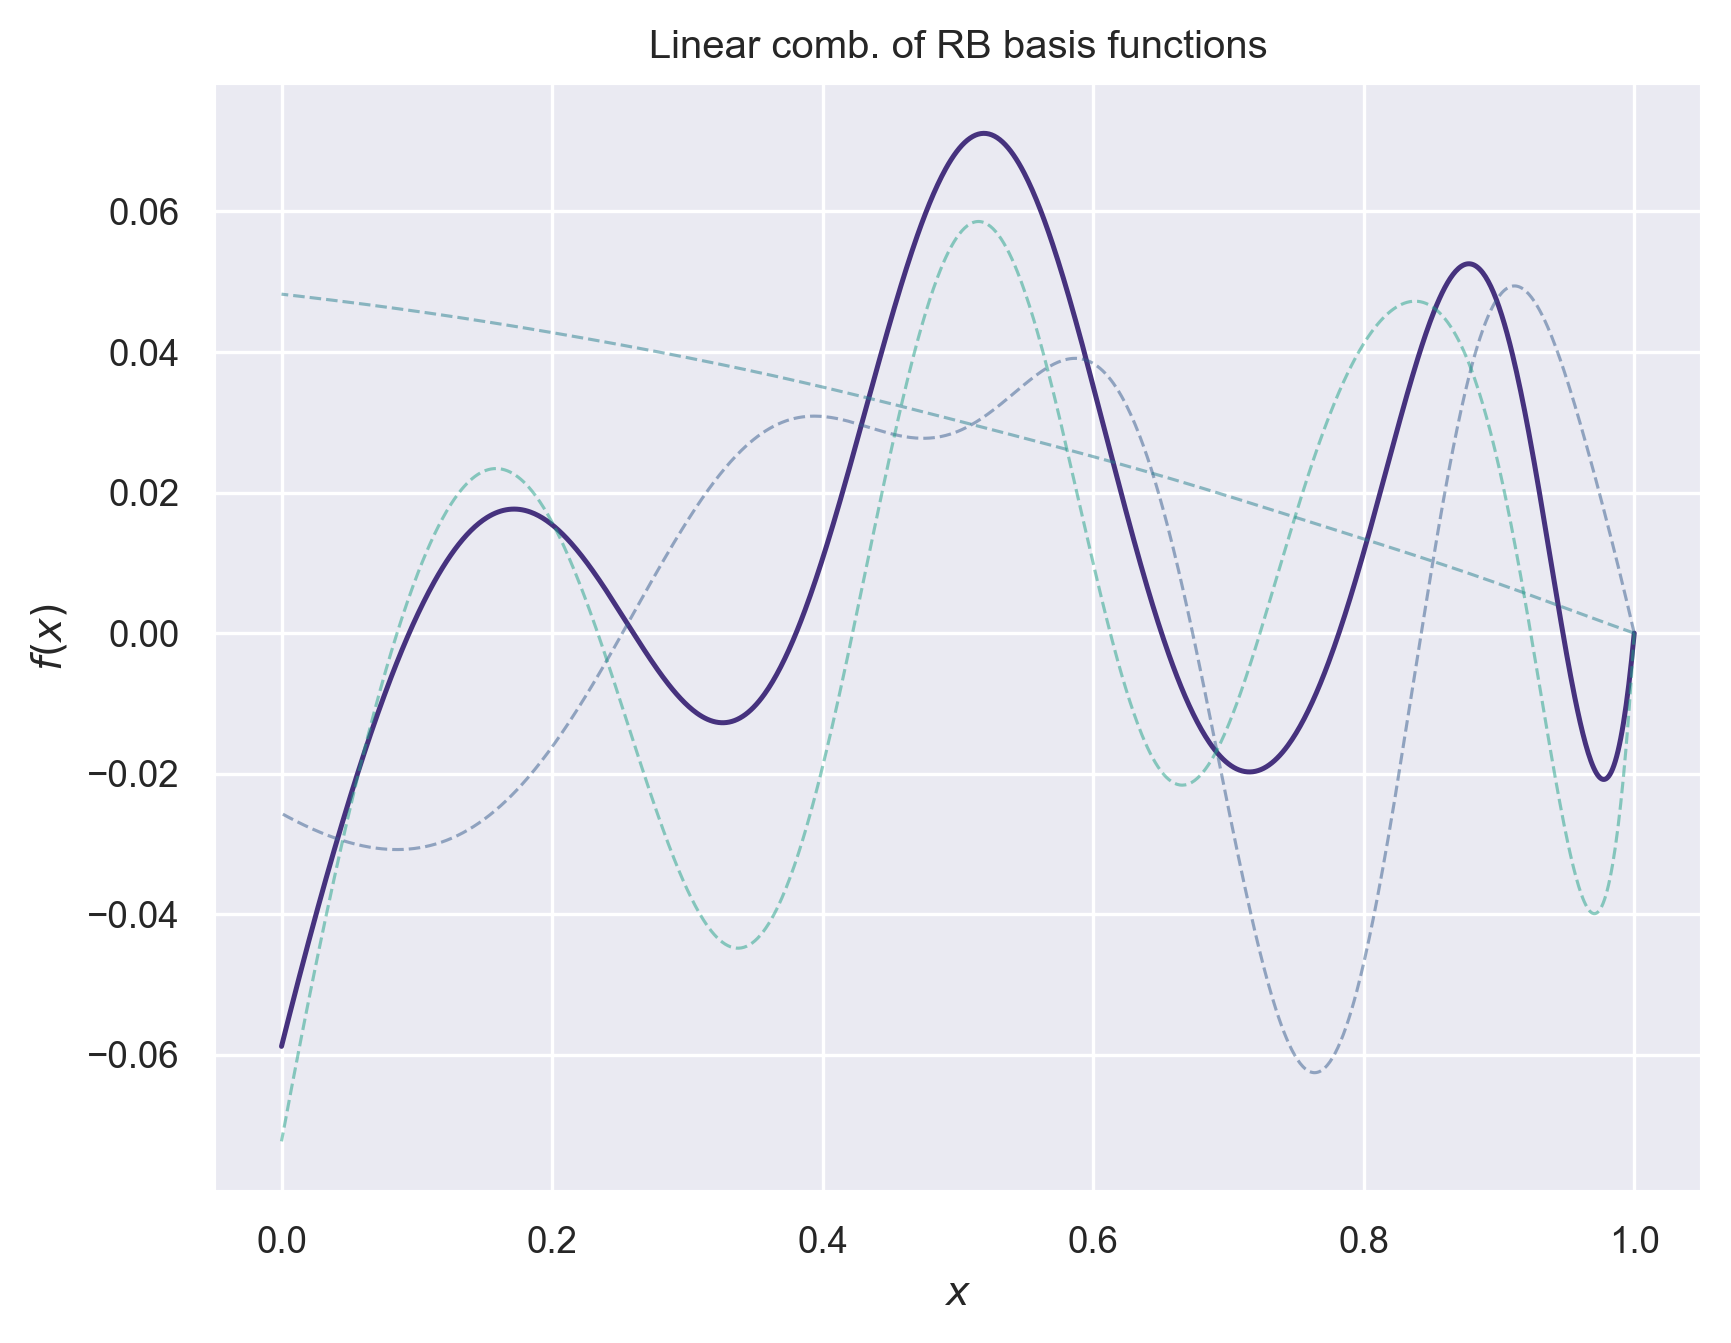
\includegraphics[width=\columnwidth]{research_project/piston/figures/svd_fourier/linear_combination.png}
    \caption{Function $f(x)$, created as a linear combination of the first three RB modes 
    from the piston problem.
    The first three RB modes are shown in dashed.}
    \label{fig:appendix_rb_linear_combination}
\end{figure}
\begin{figure}[h]
    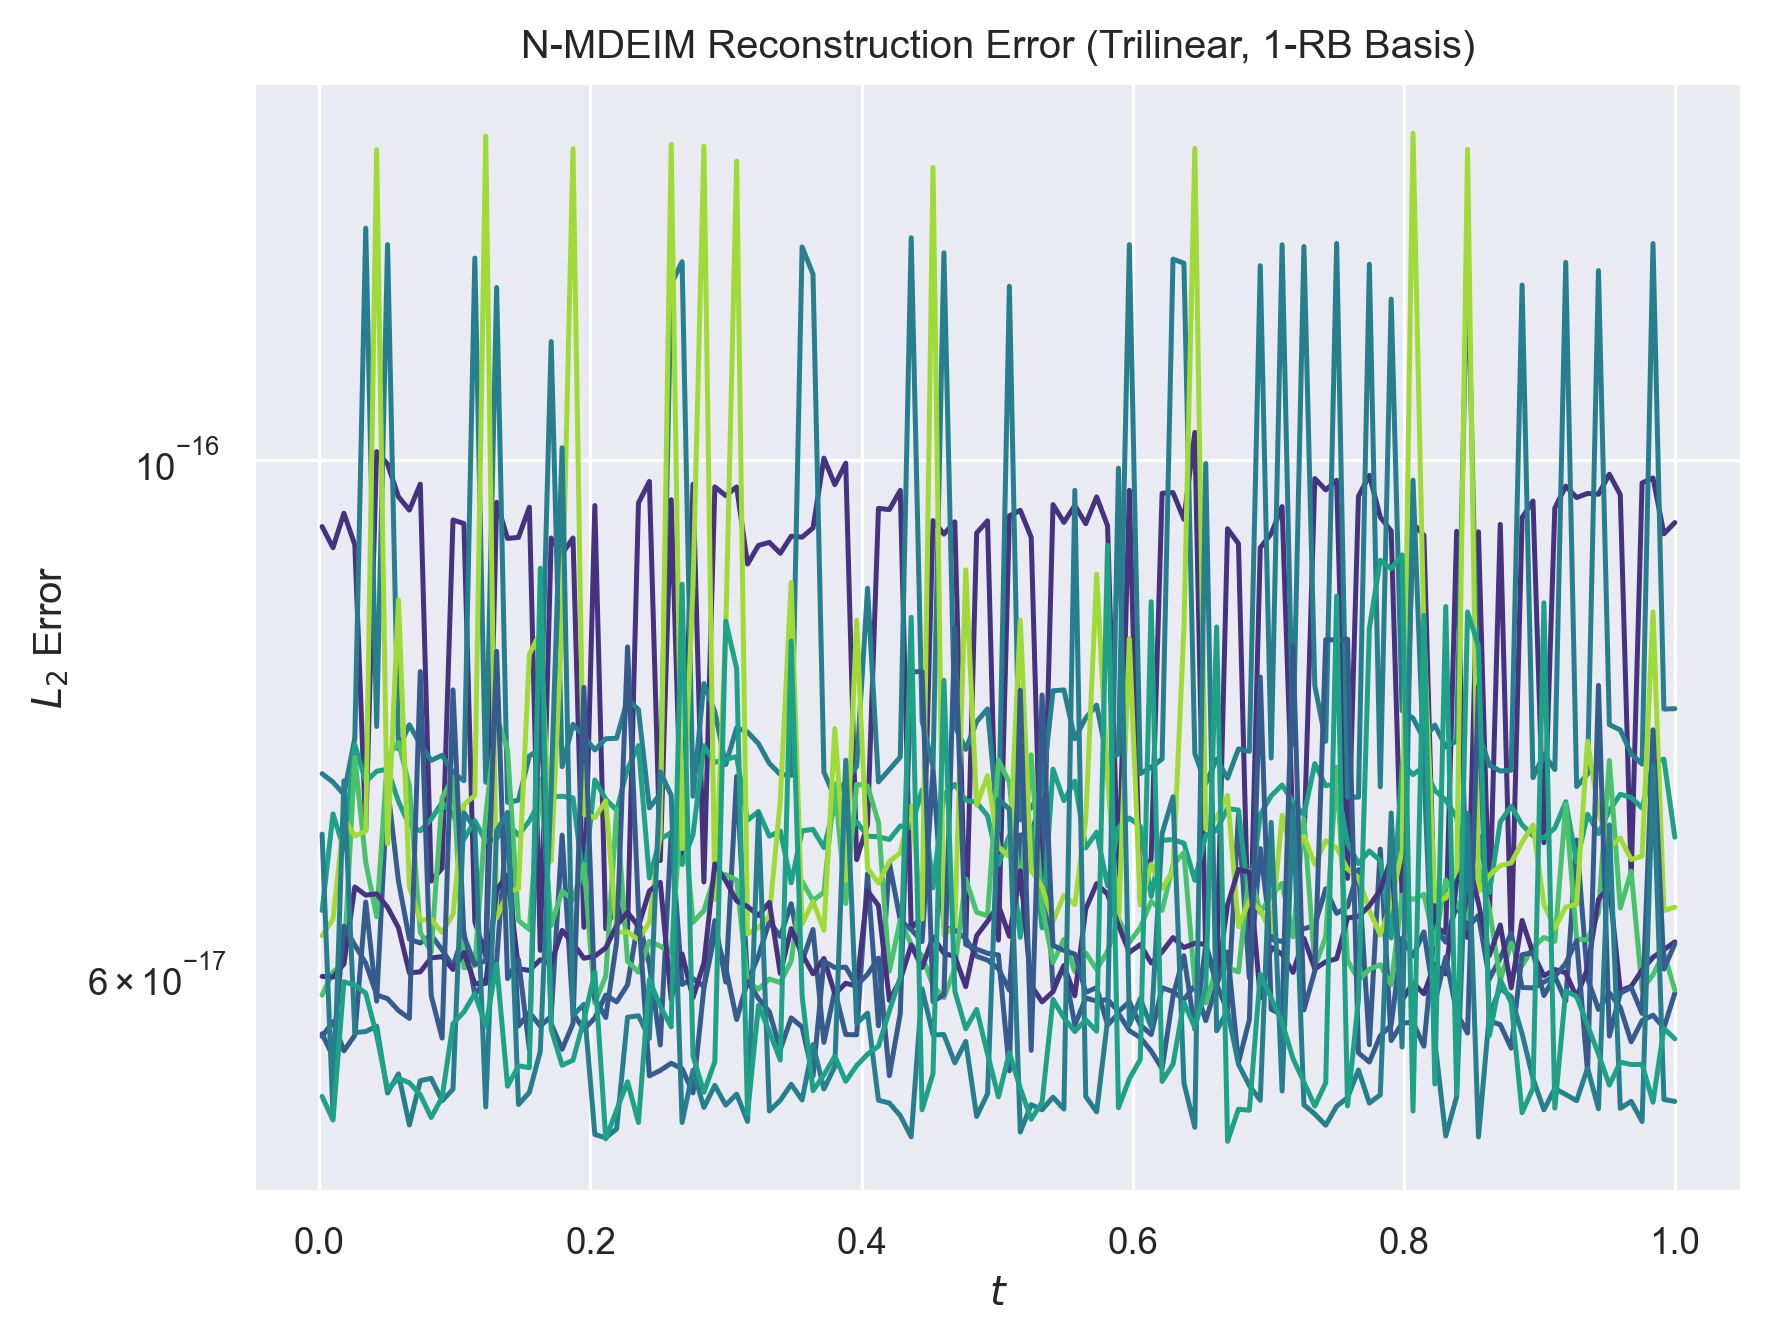
\includegraphics[width=\columnwidth]{research_project/piston/figures/svd_fourier/trilinear_nonlinear/rb_basis_mdeim_errors_trilinear_num_1.png}
    \caption{Reconstruction error for the trilinear operator evaluated with function $f(x)$.
    The basis has been obtained only using the first RB element.}
    \label{fig:appendix_rb_trilinear_num_1}
\end{figure}
\begin{figure}[h]
    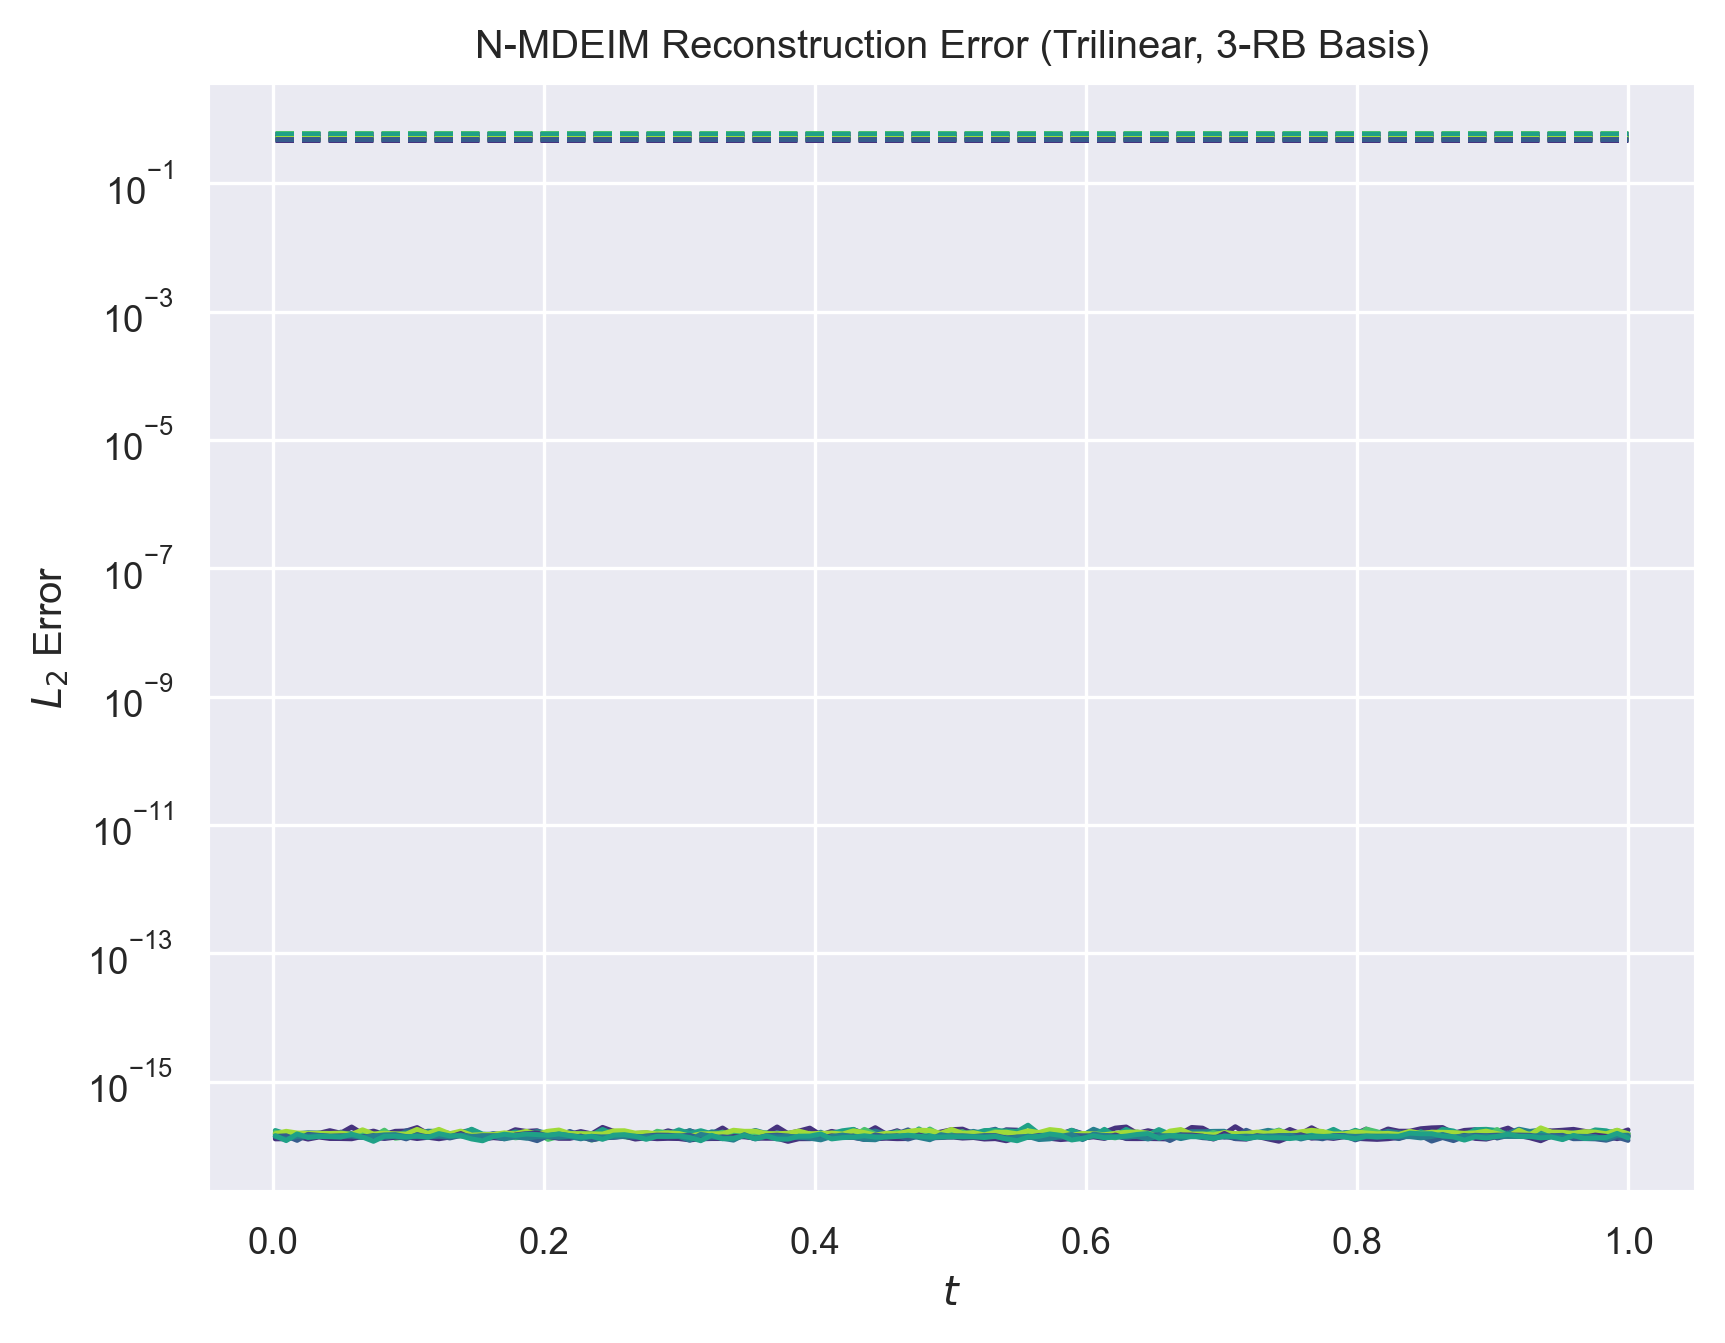
\includegraphics[width=\columnwidth]{research_project/piston/figures/svd_fourier/trilinear_nonlinear/rb_basis_mdeim_errors_trilinear_num_3.png}
    \caption{Reconstruction error for the trilinear operator evaluated with function $f(x)$.
    The basis has been obtained using the three RB element.
    In dashed is the approximation error using a truncated basis ($N=2$). 
    The truncated basis fails because the original basis is non-hierarchical, 
    hence all the elements are required.}
    \label{fig:appendix_rb_trilinear_num_3}
\end{figure}

\subsection{N-MDEIM with a Nonlinear Jacobian}
We have shown in the previous section how, 
for trilinear forms under linear Jacobian transformations, 
one can achieve a perfect collateral basis for the trilinear using exclusively one RB element.

We now explore what would happen if the Jacobian had been nonlinear instead,
or if any nonlinear operation took place inside the weak form.
Hence, we approach the reduction of
\begin{equation}
    \begin{split}
        \qty[\Ah{W}\left(\psi_{h}\right)]_{i,j}
        &= b_0 \inner{\psi_h(x) \cos(1+x) \grad \varphi_j}{\varphi_i}^{n+1},
        \\[2mm]
        &= b_0 \int_{0}^{L(t^{n+1})} \psi_h(x) \cos(1+x) \grad \varphi_j \varphi_i \dd x.
    \end{split}
\end{equation}
The results are shown in Figures~\ref{fig:appendix_rb_nonlinear_num_1} 
and~\ref{fig:appendix_rb_nonlinear_num_3}.
Both figures include the reconstruction error for a truncated base.

We find out that in the presence of a nonlinearity it is unsufficient to use only 
one basis element of the function space. 
When the basis built with approach (a) is truncated, the approximation error goes up by a lot,
leading to poor reconstruction results.

Instead, when the whole basis of the function space is used to build the collateral basis,
truncating the outcome leads to a feasible basis. 
The truncation leads to a higher approximation error, but still sufficiently small to produce
meaningful results if used in a simulation.    

\begin{figure}[h]
    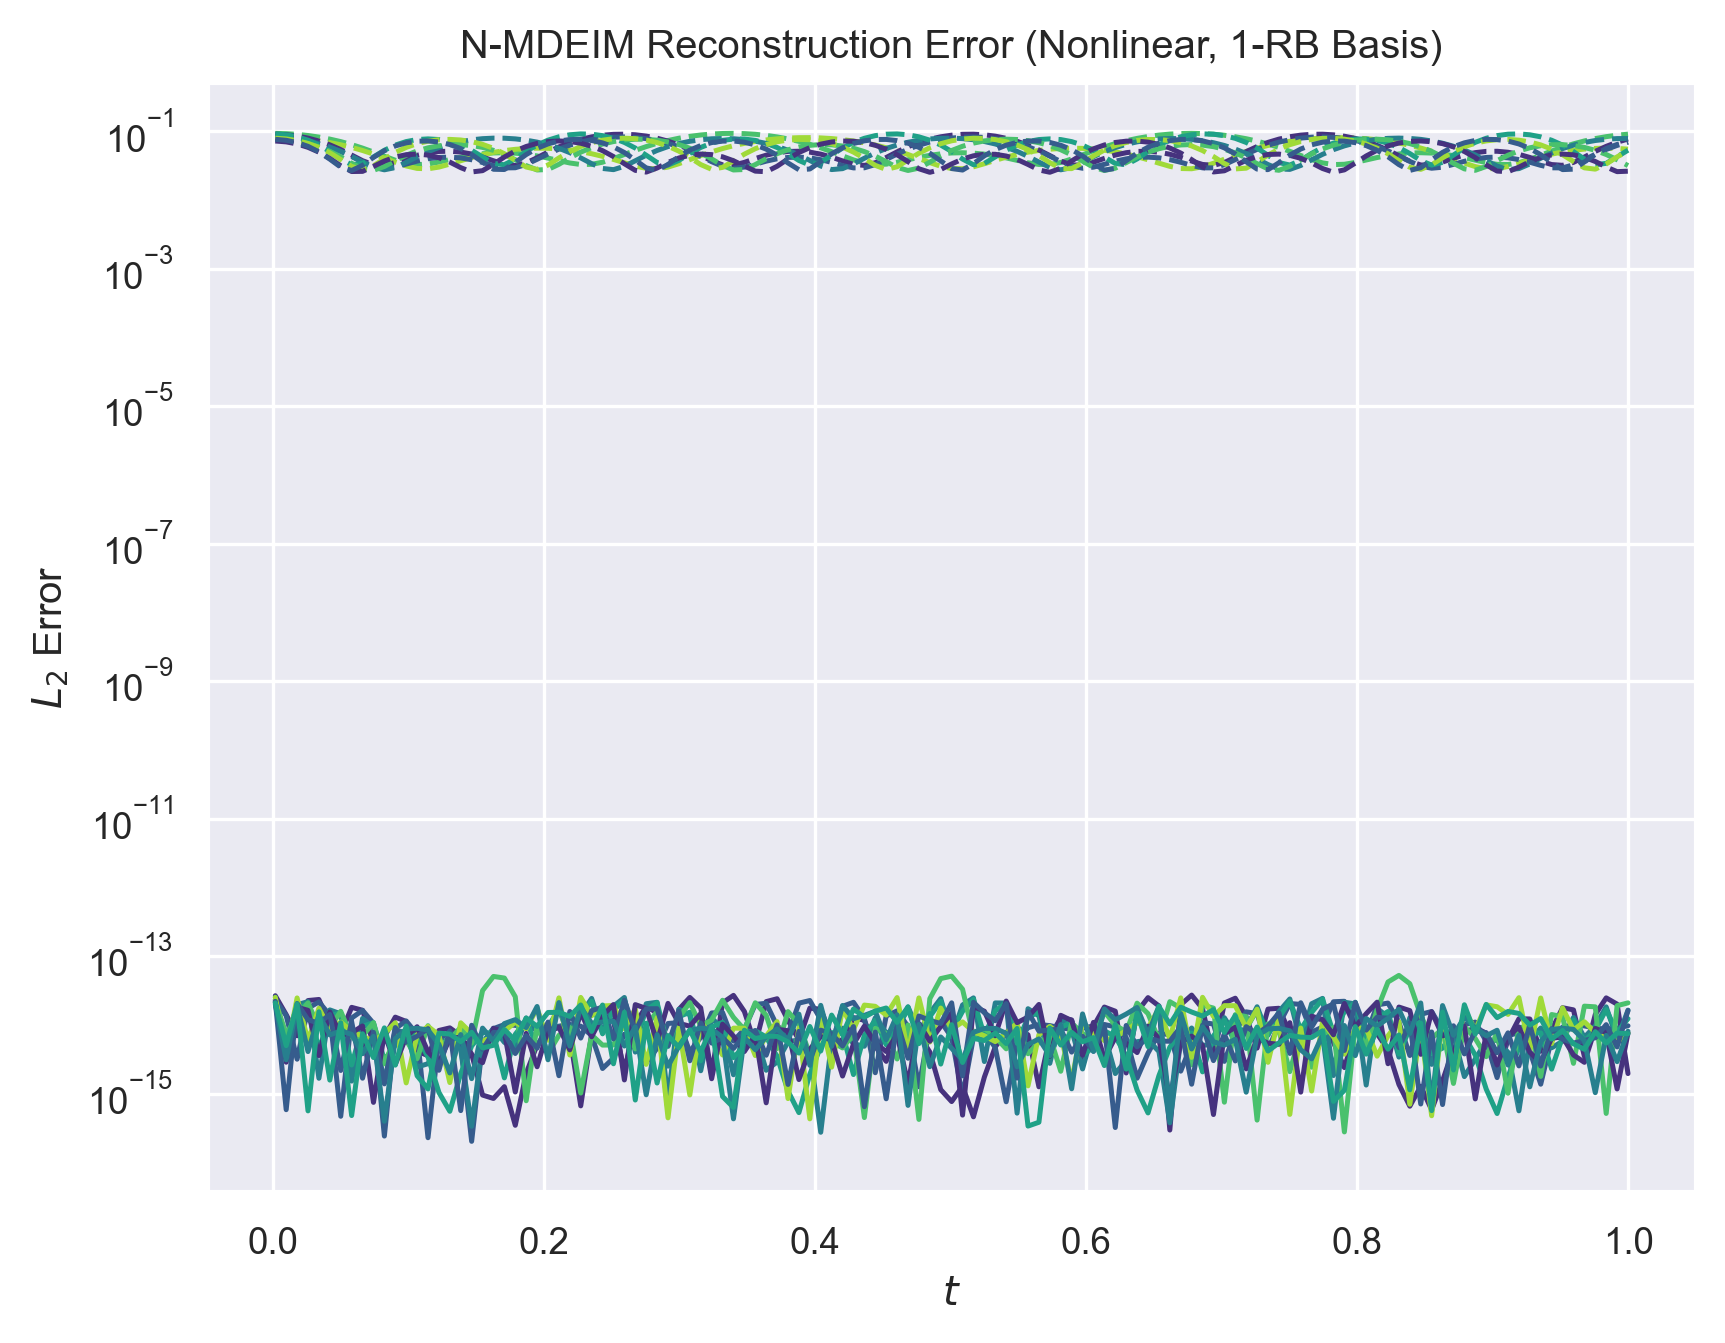
\includegraphics[width=\columnwidth]{research_project/piston/figures/svd_fourier/trilinear_nonlinear/rb_basis_mdeim_errors_nonlinear_num_1.png}
    \caption{Reconstruction error for the nonlinear operator evaluated with function $f(x)$.
    The basis has been obtained only using the first RB element ($N_{\text{full}}=7$).
    In dashed is the approximation error using a truncated basis, 
    from which only one mode has been removed ($N_{\text{truncated}}=6$). 
    The truncated basis fails because due to the presence of the nonlinearity, 
    it is now unsufficient to use only one RB basis function 
    to construct a collateral basis which accurately represents the whole space.}
    \label{fig:appendix_rb_nonlinear_num_1}
\end{figure}
\begin{figure}[h]
    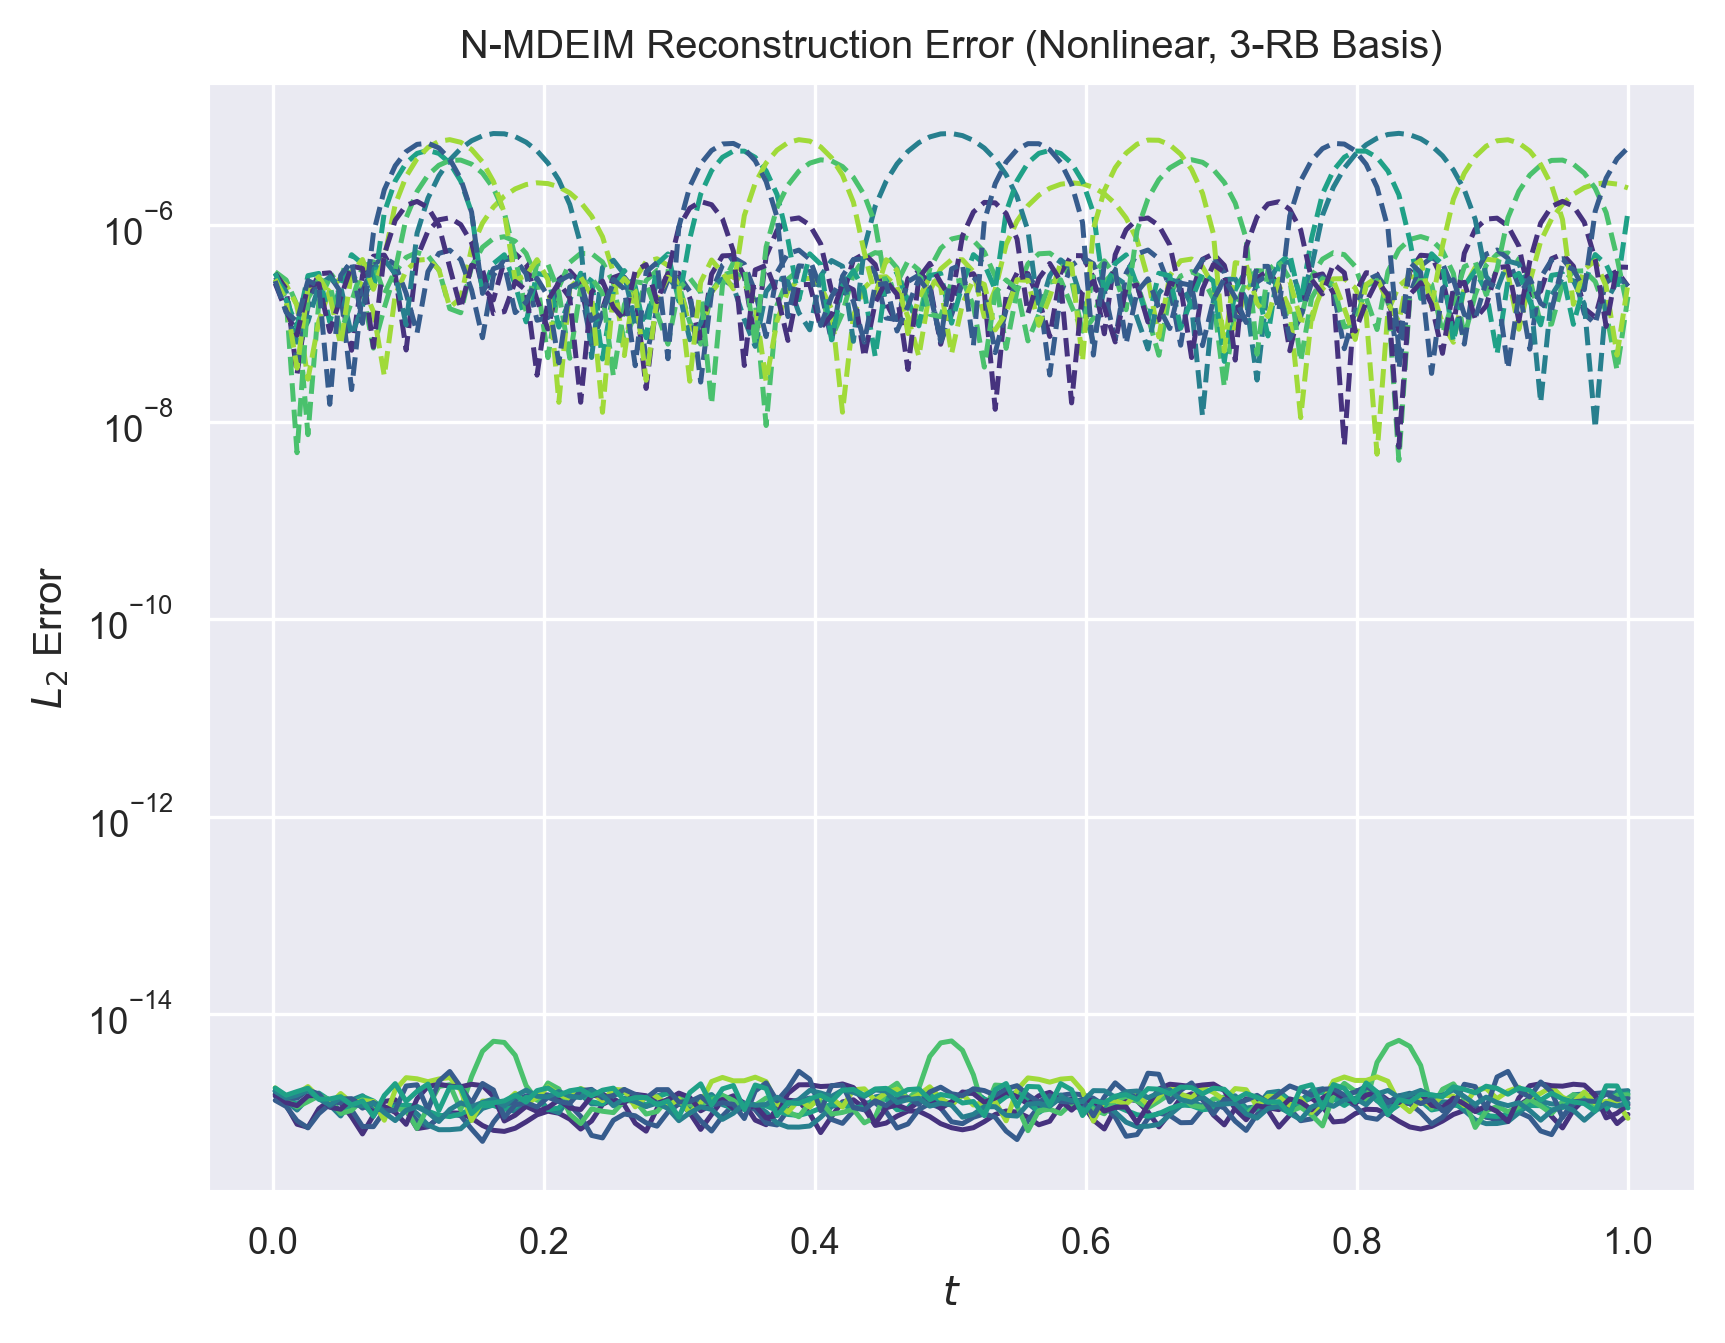
\includegraphics[width=\columnwidth]{research_project/piston/figures/svd_fourier/trilinear_nonlinear/rb_basis_mdeim_errors_nonlinear_num_3.png}
    \caption{Reconstruction error for the nonlinear operator evaluated with function $f(x)$.
    The basis has been obtained using the three RB element ($N_{\text{full}}=19$).
    In dashed is the approximation error using a truncated basis, 
    from which several modes have been removed ($N_{\text{truncated}}=10$). 
    The truncated basis does not fail as the previous ones did, it simply presents a higher error,
    but still acceptable.}
    \label{fig:appendix_rb_nonlinear_num_3}
\end{figure}

\subsection{Conclusions}
We have clarified the behaviour of the POD in the presence of a trilinear form 
and a linear Jacobian transformation.

Our first conclusion was that the POD of an orthogonal basis will produce
another orthogonal basis, as a linear combination of the input vectors.

This orthogonality is preserved under the linear transformation of the trilinear form
and the linear Jacobian.
As a consequence, the construction of the collateral basis can be achieved 
collecting snapshots with the evaluation of the trilinear form with 
only one RB basis element.
If more RB elements are used to build the snapshots, 
the POD will return a larger collateral basis,
but one that will not have a hierarchical property.
That is, truncating that basis will consistently lead to poor approximation results.
The full basis will have to be used.

Instead, under a nonlinear transformation, 
which could be present due to a nonlinear Jacobian,
the reduction trick of using one RB element is unsufficient.
All the RB elements have to be used to obtain a collateral basis that appropriately spans the whole domain.
This basis will be hierarchical, and will allow for error control through basis truncation.

If we were to collect snapshots of the operator with the nonlinear Jacobian evaluated with the PDE solutions,
we would be coupling the reduction of the RB space and the operator space.

Hence, under all conditions it is best to reduce trilinear forms using the obtained RB space.
If the trilinear form does not contain any spatial or time nonlinearity, one RB element will be enough.
Instead, if nonlinearities are present within the integrand, all the RB elements will be necessary 
to build a satisfactory basis.
One way or the other, this approach will reduce the number of snapshots to collect and compress,
leading to a lighter offline stage.
We recall that the nonlinearity can be present implicitly, 
as would happen if we assemble the matrix entries in the physical space under nonlinear mesh displacements effects.


% \subsection{Nonlinear Trilinear Form}
% Our last test is to introduce an actual nonlinearity in the trilinear form.
% We square the convective velocity term,
% \begin{equation}
%     \begin{split}
%         \qty[\Ah{W}\left(\psi_{h}\right)]_{i,j}
%         &= b_0 \inner{\psi^2_h(x)\grad \varphi_j}{\varphi_i}^{n+1},
%         \\[2mm]
%         &= b_0 \int_{0}^{L(t^{n+1})} \psi^2_h(x) \grad \varphi_j \varphi_i \dd x,
%         \\[2mm]
%         &= b_0 \int_{0}^{L(t^{n+1})} \qty(\sum_k \psi_k \varphi_k(x))^2 \grad \varphi_j \varphi_i \dd x.
%     \end{split}
% \end{equation}
% so that the input function is no longer linearly separable in its FE coefficients,
% \begin{equation}
%     \qty(\sum_k \psi_k \varphi_k(x))^2 
%     = 
%     \sum_k \qty(\psi_k \varphi_k(x))^2
%     +
%     2 \sum_{k \neq r} \psi_k \psi_r \varphi_k(x) \varphi_r(x),
% \end{equation}
% so we expect at least the necessary number of basis elements to be different from one.

